\let\negmedspace\undefined
\let\negthickspace\undefined
\documentclass[journal]{IEEEtran}
\usepackage[a4paper, margin=10mm, onecolumn]{geometry}
\usepackage{lmodern} % Ensure lmodern is loaded for pdflatex
\usepackage{tfrupee} % Include tfrupee package

\setlength{\headheight}{1cm} % Set the height of the header box
\setlength{\headsep}{0mm}  % Set the distance between the header box and the top of the text

\usepackage{gvv-book}
\usepackage{gvv}
\usepackage{cite}
\usepackage{amsmath,amssymb,amsfonts,amsthm}
\usepackage{algorithmic}
\usepackage{graphicx}
\usepackage{float}
\usepackage{textcomp}
\usepackage{xcolor}
\usepackage{txfonts}
\usepackage{listings}
\usepackage{enumitem}
\usepackage{mathtools}
\usepackage{gensymb}
\usepackage{comment}
\usepackage[breaklinks=true]{hyperref}
\usepackage{tkz-euclide} 
\usepackage{listings}
% \usepackage{gvv}                                        
\def\inputGnumericTable{}                                 
\usepackage[latin1]{inputenc}                                
\usepackage{color}                                            
\usepackage{array}                                            
\usepackage{longtable}                                       
\usepackage{calc}                                             
\usepackage{multirow}                                         
\usepackage{hhline}                                           
\usepackage{ifthen}                                           
\usepackage{lscape}
\usepackage{tikz}
\usetikzlibrary{patterns}

\begin{document}

\bibliographystyle{IEEEtran}
\vspace{3cm}

\title{10.7.8}
\author{EE25BTECH11064 - Yojit Manral}

\maketitle
% \maketitle
% \newpage
% \bigskip
{\let\newpage\relax\maketitle}
\renewcommand{\thefigure}{\theenumi}
\renewcommand{\thetable}{\theenumi}
\setlength{\intextsep}{10pt} % Space between text and float

\textbf{Question:}\\
The area (in sq. units) of the quadrilateral formed by the tangents at the end points of the latera recta to the ellipse $\frac{x^2}{9} + \frac{y^2}{5} = 1$ is
\begin{enumerate}[label=(\alph*)]
\begin{multicols}{4}
    \item $\frac{27}{2}$
    \item $27$
    \item $\frac{27}{4}$
    \item $18$
\end{multicols}
\end{enumerate}

\textbf{Solution:}\\
$\rightarrow$ The parameters of the given conic are
\begin{align}
    \vec{V} = \myvec{5/9&0\\0&1}\text{, } \vec{u} = 0\text{, } f = -5
\end{align}
$\rightarrow$ Also, using eigenvalue decomposition
\begin{align}
    \vec{P} = \myvec{1&0\\0&1}\text{, } \vec{D} = \myvec{5/9&0\\0&1} \implies \lambda_1 = 5/9\text{ and } \lambda_2 = 1
\end{align}
$\rightarrow$ This gives us very useful information
\begin{align}
    e &= \sqrt{1-\frac{\lambda_1}{\lambda_2}} = \frac{2}{3} \\
    \vec{F} &= \pm e\sqrt{\frac{\vert\vec{u}^T\vec{V}^{-1}\vec{u}-f\vert}{\lambda_2(1-e^2)}}\vec{e_1} = \pm\myvec{2\\0}
\end{align}
$\rightarrow$ Given that the points of contact are the end points of the latera recta. In the first quadrant, we have
\begin{align}
    \vec{q} = \myvec{2\\5/3}
\end{align}
$\rightarrow$ If the point of contact is $\vec{q}$, the equation of tangent to the conic is
\begin{align}
    (\vec{V}\vec{q}+\vec{u})^T\vec{x} + \vec{u}^T\vec{q} + f = 0\\
    \implies \myvec{2&3}\vec{x} = 9 
\end{align}
$\rightarrow$ Thus, we get the area of the quadrilateral in the $1^{st}$ quadrant to be
\begin{align}
    \Delta_1 &= \text{Area of }\triangle = \frac{1}{2}x_{int}y_{int} = \frac{1}{2}\times\frac{9}{2}\times3 \\
    \Delta_1 &= \frac{27}{4} sq. units
\end{align}
$\rightarrow$ Since an ellipse has a two-fold symmetry, total area of the quadrilateral must be $4$ times the area in the $1^{st}$ quadrant
\begin{align}
    \Delta_{Total} = 4\times\Delta_1 = 27 sq. units
\end{align}
$\rightarrow$ Therefore, (b) 27 is the correct option
\begin{figure}[h!]
   \centering
   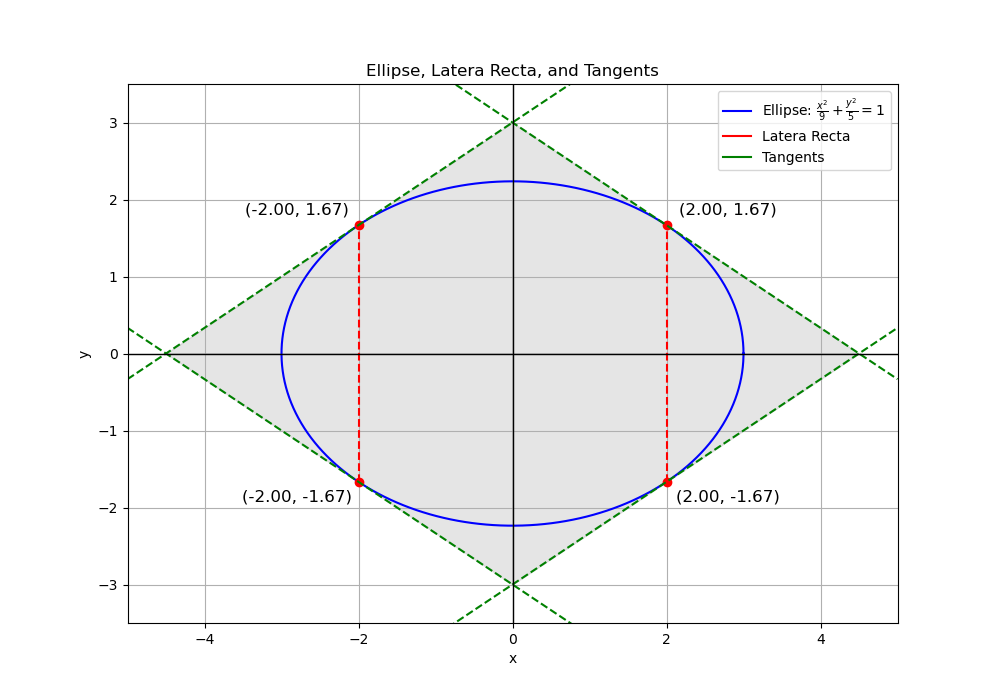
\includegraphics[width=\linewidth]{figs/01.png}
   \caption{Plot of ellipse and quadrilateral}
   \label{Plot_1}
\end{figure}
\end{document}
